\chapter{Design}
%\label{cha:part3}

\begin{comment}
Chapter 3: Design
This chapter starts to describe the student's own work. It is where the main design aspects of the project are described. The style of presentation may reflect the life cycle of the project, for example commencing with the Requirements Analysis, but it should not read like a diary. The design should be clearly and precisely described with supporting diagrams. The presentation should be at a fairly high level without excessive detail. This chapter is a suitable place to justify your choice of architecture, implementation technologies and APIs used.
\end{comment}

\plan{This section contains my PLAN of what I will do (before I started) of my app, it should be programming language independent}

This chapter covers design of the system, including an overview of the architecture and descriptions of the key components. 

\section{Statement Management}
The statement management features of the application were selected based on the functionality observed during the background research and conversations with potential users, asking what functionality they would find useful in such an application.

The key features are; parsing of files downloaded from Internet banking, mapping transactions found in the files to real world businesses and 

\subsection{Upload}
\plan{Parsing QIF/OFX, dates being bitches etc...}

\subsection{Named Entity Resolution}

\plan{Must mention what  are}

\subsubsection{Mapping to Entities}
A key part of the project is mapping the text found on a bank statement that represents a business or person to a single entity in the application. After a cleanup of different suffixes that banks append it was found that transactors are often referenced using several names.

Seen in Table \ref{tab:sainsburys}, Sainsbury's was referred to nine different ways in the statement data uploaded by the research participants and similar results are found for most \glspl{transactor}.

\begin{table}[h]
\centering
% SELECT name,count(t.id) as count FROM `transaction` AS t LEFT JOIN global_transactor_mapping AS g ON global_transactor_mapping_id = g.id WHERE global_transactor_mapping_id IN(SELECT id FROM global_transactor_mapping WHERE transactor_id = 7) GROUP BY global_transactor_mapping_id ORDER BY count DESC
\begin{tabular}{@{}ll@{}}
\toprule
Reference            & Occurrences \\ \midrule
sainsburys s/mkts    & 46          \\
sainsburys s/mkt     & 9           \\
sainsburys s/mkts cd & 7           \\
js online grocery    & 2           \\
sainsbury s/mkt      & 2           \\
sainsburys smkt      & 2           \\
js online grocer     & 1           \\
sainsburys superma   & 1           \\
sainsburys-superma   & 1           \\ \bottomrule
\end{tabular}
\caption{References to the same entity `Sainsbury's' found in participant data}
\label{tab:sainsburys}
\end{table}

In consideration of this, the concept of mappings were added to the system. A mapping is a single reference to a transactor, such as `sainsbury s/mkt'. A transactor has multiple mappings. Fig. \ref{fig:mapping} shows this structure.

\begin{figure}[h]
    \centering
    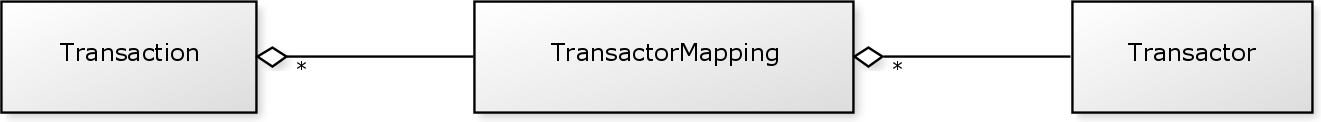
\includegraphics[width=\textwidth]{simple-mappings}
    \caption{Overview of Mappings}
    \label{fig:mapping}
    
    \begin{comment}
%[User]-*<>[Transaction]
[Transaction]<>*-[TransactorMapping]
[TransactorMapping]<>*-[Transactor]
    \end{comment}
\end{figure}


\subsubsection{Global vs User}
Early on it became clear that users should be able to categorise and organise transactions according to their preferences, however categories chosen by a particular user should not affect affect other users.

To support this the application stores two sets of mappings and transactions, User and Global. The structure of the relevant objects is shown in Fig. \ref{fig:transactormappings}. A Transaction can have both a UserMapping and a GlobalMapping, in which case the UserMapping overrides the GlobalMapping when calling methods such as \inlinephp{getMapping()} on the Transaction.

\begin{figure}[h]
    \centering
    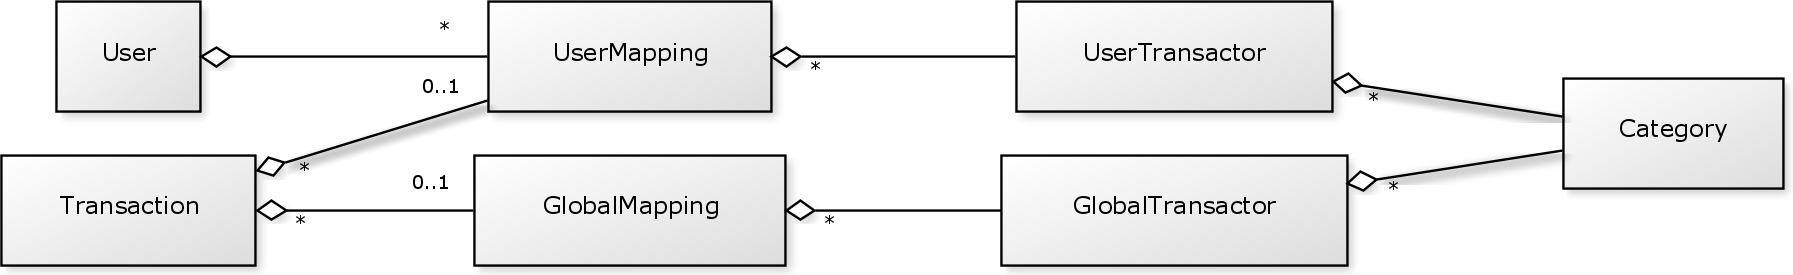
\includegraphics[width=\textwidth]{mappings}
    \caption{Overview of User Mappings}
    \label{fig:transactormappings}
    
    \begin{comment}
[Transaction]<>*-0..1[UserMapping]
[Transaction]<>*-0..1-[GlobalMapping]
[User]<>-*[UserMapping]
[UserMapping]<>*-[UserTransactor]
[UserTransactor]<>*-[Category]
[GlobalTransactor]<>*-[Category]
[GlobalMapping]<>*-[GlobalTransactor]
    \end{comment}
\end{figure}



\plan{Use of MySQL to find similar, how that works, alternatives}

\subsection{Suggestions}
\plan{How it uses the above, how the whole user/global thing works}

\section{Prediction}



\subsection{Prediction}
\plan{All the steps that were needed for the prediction}

\subsection{Markov Chain}
\plan{Why I chose first order markov chains, alternatives to that etc...}

\subsection{Weighted Averages}
\plan{How does that work, why is it good?}

\subsection{5 Model System}
\plan{How was is a model chosen for the user?}

\section{Security Considerations}
\todo[inline]{Make this section make sense}
Strong security is of high importance this project, the design considered possible attack vectors and took steps to prevent of reduce the effectiveness of those attacks.

\subsection{Account Hijacking}

Over HTTP information sent between the users web browser and the remote server is sent in plain text. The weakness of this is only enhanced when accessing the internet using an unencrypted wifi connection which would allow anyone in the local area to `sniff' the information sent between the browser and the internet by simply scanning and downloading the packets transmitted.

Although this is a serious security risk this only gets worse when the website involves authentication. Authentication is usually performed by sending the userame and password in plain text to a remote server, which is validated and if correct the user is issued with a session cookie.

A potential attacker could observe and store these usernames and passwords, which is why websites including Facebook used HTTPS for the login, ensuring the usernames and passwords were sent encrypted. 

However, there is still a security flaw if the website falls back to HTTP following the authentication. To prove to the server which website the user represents the user sends their cookie containing a secure ID to the remote server with each request. Although the attacker was unable to sniff the username and password they can perform a session hijack by downloading the content of that cookie to their local machine and prove that they are the user to the remote server accessing all of their data. 
% 
Firesheep was a proof of concept plugin for Firefox released in 2010 that demonstrated this vulnerability, showing that session hijacking could be performed on popular sites including Google, Facebook, Twittter and Flickr, which until recently were not using sidewide SSL.
%http://codebutler.com/firesheep/ FireSheet mention, http://codebutler.github.io/firesheep/

For this reason all of the application uses HTTPS, and redirects users to the HTTPS version if they attempt to access HTTP. This ensured user data is encrypted end to end and cannot be sniffed and neither can their authentication details or session cookie.

\subsection{Password Security}

A common way to crack into user accounts is by brute force. If an attacker knows a particular users username they can perform targeted guessing guessing of the password by enumerating through all possibilities. A websites ability to resist this kind of attack is called the `password guessing resistance'. It is for this reason that many websites, following the guidance of research such as \cite{needed} enforce password rules in an attempt to increase the number of possible combinations for a password, the entropy.

Shannon Entropy can be used estimate the strength of a passwords resistance to this kind of attack. The entropy is calculated using $H(X)= - \sum_{i=1}^n{p(x_i)\log_b p(x_i)}$ where $p(x_i)$ is the probability of the value $x$ occurring \cite{burr2013electronic}.

The paper suggests a predefined set of rules for estimating entropy based on Shannon's work studying English text \cite{burr2013electronic}, however other papers found that using this predefined set of rules was not a valid measure of password strength \cite{weir2010shannon}.
% 
The project uses Shannon's original equation, calculating the probability of guessing an individual character using a formula that takes into account that using a larger character set (such as numbers and symbols) decreases the likely hood of successfully guessing the next character.

As part of a brute force, an attacker may use a dictionary of popular passwords to reduce the testing space before attempting an exhaustion attack. In order to reduce the effectiveness of this kind of attack the project test's any user provided password against a dictionary of at least 50,000 common passwords sourced from password cracking resources \cite{burr2013electronic}.

In addition, to limit the overall effectiveness of brute force attacks, the website rate limits login attempts. If a user attempts to login more than 5 times within one minute, they must wait a minute before they are able to login again.

\subsection{Database Storage}
Unfortunately, it's common for the contents of a websites database to be leaked, whether by an administrator of the website or using other techniques such as SQL injection. It's important to think about the security of the data held within the database, as well as the security of the front end.

pegFinance uses three main techniques to help ensure the security of the users information in the database.

\subsubsection{Passwords}
A users password should never be kept in a reversable state, whether that is plain text\footnote{Unfortunately still very common} or encrypted\footnote{Also common}. If a database of encrypted or plain text passwords is leaked, it is simply a case of finding the encryption key and all the data can be accessed in plain text.

This is why standard security practice is to hash (one-way) passwords. The only way to decrypt a one-way hash is to guess the original input by brute force and see if that matches the output.

However attackers often use of Rainbow tables, collections of precalculated hashes and the input used to create them, allowing an attacker to simply lookup a hash in their database to get the result.

For this reason salting is used, which involves adding a random collection of numbers and letters to each password. This means that the generated hash is dependent on both the users password and the salt and means a Rainbow Table would need to be generated for each user, mitigating the effect.

There is a final step and that's what hashing schema should be used to hash passwords. Traditionally functions such as MD5, SHA1 and SHA256 were used to perform the hashing, however due to advances in modern computer equipment it is possible to generate these at an incredibly fast rate, reducing the time taken to brute force a hash.

Using a deliberately slow hashing function is designed avoid this problem. Blowfish written by Schneier is commonly suggested, as it is designed as a computationally expensive operation. This was demonstrated with a simple test, calculating as many hashes per possible in one second. Table \ref{tab:hashspeed}, shows the results, which found that on average Blowfish took significantly longer to generate each hash.

For this reason the project salts all passwords and hashes them using Blowfish.

\begin{table}[h]
\begin{tabular}{llll}
         & \multicolumn{3}{l}{Hashes Per Second}                   \\
         & Average & Standard Deviation & 95\% Confidence Interval \\
MD5      & \num{2296667} & \num{12923}              & $\pm 8010$                 \\
SHA1     & \num{1869725} & \num{14783}             & $\pm 9162$                 \\
BLOWFISH & 17      & 0                   & $\pm 0$                    \\
\end{tabular}
\label{tab:hashspeed}
\caption{Average number of hashes completed per second on a 2.7Ghz i7 }
\end{table}

\section{Technical Design}

\subsubsection{Personally Identifiable Data}
Of equal concern is other personally identifiable data being leaked, in an attempt to avoid this the application encrypts all information stored in the user table, that is needed at a later date using the AES128 encryption standard. This standard was selected for the project as was endorsed by the U.S. National Institute of Standards and Technology, when outlined by NIST in 2001 and has become the ``encryption standard for commercial transactions in the private sector'' \cite{nist2010aes, stair2009informationsystems}.

\subsubsection{Hashing of Username}
In addition to the above the username of each user is also hashed so it is only known to the person using that account. In the rare case that any of the passwords were brute forced, the relevant username would also need to be brute forced in order to attempt to login or use the details on another website.

\subsection{Other}
Other attack vectors inclung SQL injection and cross-site scripting (XSS) were also considered.

It was decided that the project would use a prepared statements to reduce the risk of SQL injection. By sending the query followed by the parameters as literal values the database server would not interpret them as an executable portion of SQL and attacks, relying on escaping SQL such as \inlinesql$' OR 1$ are prevented.

In order to mitigate the possiblity of XSS the project will need escape all content before displaying it to the user or saving to the database. It was decided that the project would use a templating language that escaped output by default, requiring the output be explicitly marked to avoid escaping. By escaping all content before displaying it to the user a maliciously crafted piece of text such as \inlinehtml$<script>alert(1);</script>$ would be sent to the users browser as \inlinehtml$&lt;script&gt;alert(1);&lt;/script&gt;$ and not interpreted as a script.

\section{Technical Design}

\subsection{Object Orientation}

\subsection{Domain Class}

\subsection{UI Design}

\todo[inline]{Add photos showing the evolution of the UI}



\subsection{Database Class}

\subsection{External Software and Frameworks}